
前節で紹介したRNNでは、隠れ状態$h_t$はその前の隠れ状態$h_{t-1}$と入力状態$x_t$に依存して決定される。言い換えると、データのシークエンスで表される時系列データを、データの先頭から時間に沿って再帰的に計算を行っていく。そのため、学習段階でのバッチを用いた並列処理(GPUの有効活用)が困難となるうえに、一つ手前の隠れ状態のみを使うため長期の時系列データを効率よく学習できないという問題点もある。詳しくは前節を参照してほしい。

transformerでは複数の機構を組み合わせることで、これらの問題に対する解決を図った。以下ではtransformerにおける重要な構成要素を一つづつ紹介していく。

% 機構は要素間の距離に関係なく依存関係をモデリング出来るという利点を持ち、様々な時系列データを用いたタスクにおいて必要不可欠なものになりつつある。


\subsubsection{エンコーダとデコーダ}
原著論文「Attention is all you need」で提唱されたtransformerはエンコーダ・デコーダ transformerと呼ばれており、その名前の通りエンコーダ層とデコーダ層の二つのサブネットワークから構成されている。このエンコーダ・デコーダ モデルは文章から文章への変換 (Sequence to Sequence、Seq2Seq)が可能であり、翻訳問題を扱う場合には、エンコーダ層で入力情報である翻訳元の言語をエンコードし、デコーダ層でそのエンコードされた情報を元に翻訳先の言語へと変換する。

transformerには他にもエンコーダ層のみを持つエンコーダtransformerやデコーダ層のみを持つデコーダtransformerも存在し、それぞれ文章生成や文章のクラスタリング問題などに用いられる。この二つもtransformerを理解する上で重要な概念ではあるが、本節では原著で紹介されているエンコーダ・デコーダtransformerに焦点を当てて解説を進めていく。


\subsubsection{Token Embedding}
上記で説明したように今回は翻訳問題を扱う。ここでの翻訳とは文章から文章への変換、例えば日本語の文章から英語の文章への変換を指す。

プログラミングを用いた自然言語処理では文章や言葉をそのまま入力として扱うのではなく、文章をトークンに分けて考える(トークン化と呼ぶ)。トークンとは単語や単語をさらに分割した単位のことを指し、英語の場合は単にスペースで文章を区切る場合が多い。例えば以下の様なトークン化が採用される。


% \begin{quote}
\begin{itemize}
\item 私の趣味はプログラミングです。$\rightarrow$ [私/の/趣味/は/プログラミング/です/]
\item My hobby is programming. $\rightarrow$ [My/Hobby/is/programming/.]
\end{itemize}

全てのデータセット(翻訳対コーパス)のトークン化が完了すると、次にコーパスの中に出現する全ての語彙(トークン)に一意な番号を割り振る。この時に割り振った番号の総数を語彙数と呼び、データセットが大きくなればなるほど語彙数が膨大になる。通常、文頭・文末には特殊なトークンが割り当てられおりそれぞれ\emph{bos}・\emph{eos}と呼ばれる。以降全ての文章はトークン化が事前に施されていると仮定する。なおこれらの作業は言語ごとに行われる。

ここで翻訳問題を数学的に定義する。

\begin{itembox}{\bf コラム 翻訳問題(seq2seq)}
  ある言語の文章を$X = [x_0, x_1, .., x_{L}]$、 別の言語の文章を$Z = [z_0, z_1, .., z_{L^\prime}]$であらわすとする。これらを用いると翻訳問題は以下の確率分布を求めることに対応する
  \begin{align}
    \Pr(X = \vc{x}|Z) = P(x_0| Z) \cdot P(x_1| Z, x_0) \cdots P(x_L| Z, x_0, \ldots x_{L-1})
  \end{align}
  最初の文字は\emph{bos}で固定されているため、実際は$x_1$から始まり文末を表す\emph{eos}が出現するまでの確率分布を求める。

  以上を踏まえて、transformerは翻訳元の文章$Z$に加えて$l-1$文字目までの翻訳先の文章$\lbrack x_0, \ldots x_{l-1} \rbrack$を入力として確率分布のベクトル
  \begin{align}
    \label{eq:trans}
    \vec{f_\theta}(\lbrack x_0, \ldots x_{l-1} \rbrack,Z) = 
    \begin{pmatrix} 
      P_\theta(x_1 | Z, x_0)\\
      P_\theta(x_2 | Z, x_0, x_1)\\ 
      \vdots\\
      P_\theta(x_l | Z, x_0, \cdots, x_{l-1} )\\
      \end{pmatrix}
  \end{align}
  を出力する関数として定義される
\end{itembox}

\vspace{5mm}
それぞれのトークンに割り振られた番号はその後、高次元空間上でのベクトルへと移される。このベクトルは学習を進めることで単語の意味を含むようになり、似た単語はお互い似たベクトルとして表されるようになりると期待される。


% \begin{align*}
%     \mathbf{W}_e &\in \mathbb{R}^{d_e\times N_V} \\ 
%     \mathbf{r} &= \mathbf{W}_e \mathbf{e}_t
% \end{align*}

\begin{equation*}
  \text{具体例}
\end{equation*}


\subsubsection{位置符号化}


% Token Embeddingを用いてトークンのリストをベクトルのリストに変更した後、これらのベクトルに対して並列処理を施す事を考える。並列処理を行うということは、一回の処理に着目するとそれぞれのベクトルの順列は重要でないことになる。しかしながら、現在のデータ形式のままではベクトルが単語同士の位置関係情報を含んでいないため、このまま並列処理を施してしまうとリスト上のベクトル同士の位置関係を区別できない。 

このモデルには再帰性も畳み込みもないので、モデルがトークンの順序を理解するために、シーケンス中のトークンの相対位置あるいは絶対位置に関する何らかの情報を埋め込む必要がある。
例えばこのまま、「トークンの集合」のみを入力として渡してしまうと、「明日の天気は晴れです。」 と 「天気の明日は晴れです。」を区別できないことになる。従って何らかの方法をもって、文章内のトークンの位置を符号化する必要がある。

例えば、最初に現れるトークンに”1”を付与し、二つ目のトークンに”2”を付与するなど、文章内でのトークンのインデックス自身を位置情報として扱う方針をとることが出来る。この方針を採用すると文章が長くなればなるほど大きい値を取るようになるが、これは幾つかの問題を内包している。一つ目は学習が不安定になるという点である。このことは、ニューラルネットワークを学習する上で、予め入力データのスケールを統一する事が重要であるという事実から理解できる。二つ目の問題点は、符号化された位置情報間の類似度に一貫性が無くなるという点である。transformerで核となるattentionではベクトル間の内積を用いてベクトル間の類似度を表現している。一方ベクトル間の内積を考えるとき、トークンの位置によって内積計算後のスケールに違いが生まれてしまうと、データの意味合いに一貫性が持てなくなる。例えば、「明日の天気は晴れです。」という一つの文をとっても、この一文が長い文章の中の最初に出てくるか最後に出てくるかで、まったくの別物として解釈される可能性がある。

それならばということで、$\lbrack1, 2, \ldots, \rbrack$と割り当てるのではなくて、0が最初の文字で1が最後の文字を表すように、値を$[0, 1]$の間にスケール変換した場合を考える。この時、文章が長くなっても1以上の値をとることは無くなるが、値だけ見ても絶対位置と相対位置が分からないという問題点が出てくる。例えば、0.1と0.2という値が位置情報として付与された二つのトークンが近くに位置するのか遠くに位置するのか判断が出来ない。

これらのことから位置符号化には以下の要求を課す。
\begin{enumerate}
  \item 文章の長さに関わらず、トークンの位置ごとに一意な値を持つ(絶対一が復元できる)。
  % \item 文章の長さに関わらず、トークンの位置ごとに一意な値を持つ。
  \item トークン間の相対距離が、トークンの位置や文章の長さによらず一貫性を持っている。
  % \item トークンの位置や文章の長さによらず、位置符号化間の類似度の意味合いが一貫性を持っている。
  \item 扱える文章の最大長を変更することが容易である。
\end{enumerate}

上の条件を満たすもので一番簡単なものは、単位円上の座標を表す二次元ベクトルを用いて位置符号化を定義する場合である(図~\ref{fig:pos-encoding-circle})。この場合、二点間の類似度は間の角度を用いて定義される。角度が$0[\text{rad}]$にある点が最初のトークンを表し、角度が$1[\text{rad}]$にある点が、扱える文章の中の最後尾を表すとする(ある文章の中の最後のトークンとは限らないことに注意)。従って隣り合う点の間の角度は$1/l_{max} [\text{rad}]$となる。ここで$l_{max}$とは、データセットの中で最長の文章が保有するトークンの数である。

\begin{figure}
  \centering
    % 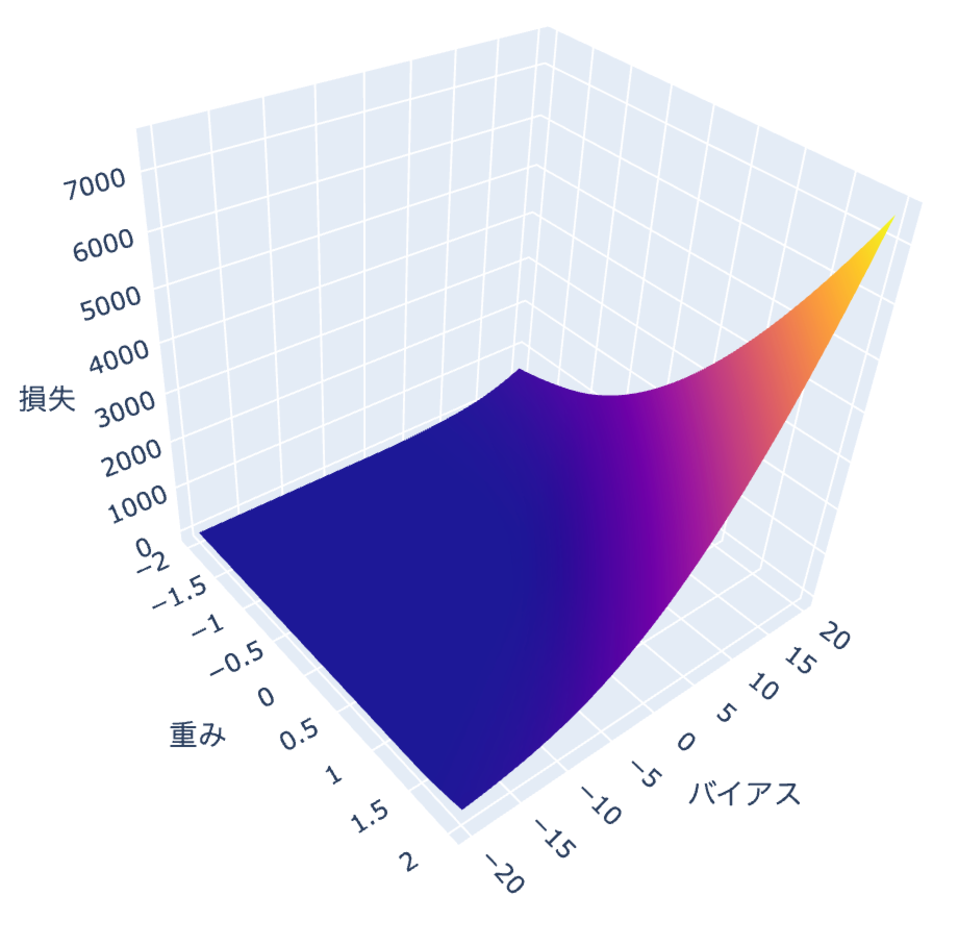
\includegraphics[width=0.7\linewidth]{fig/1-dim-relu-3d.pdf}

  \caption{二次元平面上の単位円}
\label{fig:pos-encoding-circle}

\end{figure}
実は、3つの要求さえ満たしていれば隣り合う点の角度を$1/l_{max} [\text{rad}]$よりも大きく取ることが可能であり、角度に応じてその位置符号化が得意とするスケールが変化する。例えば二点間の角度が小さい場合はより波長が長くなるため、より大きいスケールでの位置関係を符号化するのに適しているのに対し、角度が大きい場合は、より小さいスケールでの位置関係を符号化できる。これらの考察を進めると、それぞれの角度が異なるような二次元の円周を複数個用意し、それらを全て合わせたものを新しい位置符号化として表せすことで、様々なスケールの位置情報を一度に符号化できる事に気が付く。
% トークンのインデックス値そのものを用いて位置を表現する方針を取ることも出来るが、transformerでは位置情報を、token Embedding同様、高次元のベクトル空間へと埋め込む。

% 位置符号化ではトークンごとの前後関係情報を先ほどのベクトルに足し上げる。

Transformerでの位置符号化の場合はまさにこの方針を取っており、得られた位置符号化はtoken embeddingの出力結果に足し上げられる。この操作を行うことでトークンを表すベクトルは、トークン自体の意味に加えて文章中におけるトークンの位置情報も内包することになる。図~\ref{fig:tri-pos-encoding}は実際にtransformerで用いられている位置符号化をカラーマップで表現した図である。縦軸は単語の文章中における位置を表し横軸はベクトルのインデックスを表す。左に位置するほど位置の変化に敏感であり、右に位置するほど長距離の位置関係を表現している。
\begin{figure}
  \centering
    % 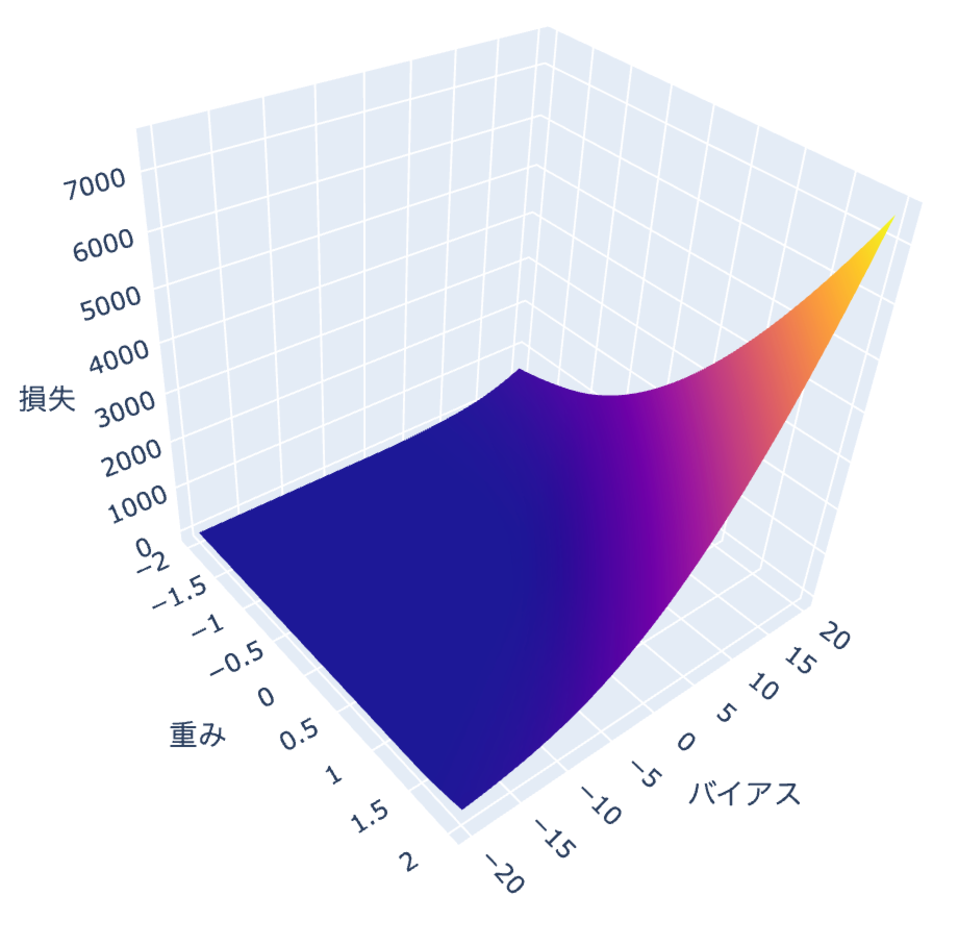
\includegraphics[width=0.7\linewidth]{fig/1-dim-relu-3d.pdf}

  \caption{三角関数を用いたToekn Encoding.}
\label{fig:tri-pos-encoding}
\end{figure}

具体的に日本語の文章「」がどの様なプロセスを辿ってtransformerに入力されるのかを、ベクトルの次元が4の場合に確認をする。


\begin{equation*}
  \text{具体例}
\end{equation*}

この様に位置符号化の適用後は、単語の意味だけでなく文章中の位置関係も一つのベクトルとして表現され、その結果それぞれのベクトル(元々はトークン)を並列的に処理できるようになる。


\subsubsection{Attention}
attentionとは文中のの特定の箇所に注意を向けるように学習していく方法である。 この関数は入力として二つの変数 x と z を受け取り、 x=z の場合を特別にself attentionと呼ぶ。例えばxとして、翻訳元である日本語のトークン列、zとしては、翻訳先である英語のトークン列が対象となる。このattentionはtransformerの肝となる部品であるがその働きは直観的であり、人間が文章を読んだり翻訳する際に自然に行っている行為を再現した機構となっている。詳しい数式の説明は省くが、前述したようにtransformerで用いられるattentionでは内積を用いた類似度計算が使用され、類似度が高いトークンに注目を集める用に学習していく。この様なattention機構のことを特に"Scaled Dot-Product Attention"と呼ぶ。図~\ref{fig:att-abs}はattentionを直感的に説明する上で役立つ概念図である。(a)のself attentionはエンコーダ層・デコーダ層の両方に埋め込まれており、文章中の単語の意味を理解する際に、文章中のどの単語に注目するべきかを学習する。デコーダ層のみに埋め込まれてる(b)は通常の意味でのattentionであり、翻訳先の文章における次の単語を生成するためには翻訳元文章のどこに注目すれば良いかを学習する。


\begin{figure}
  \centering
    % 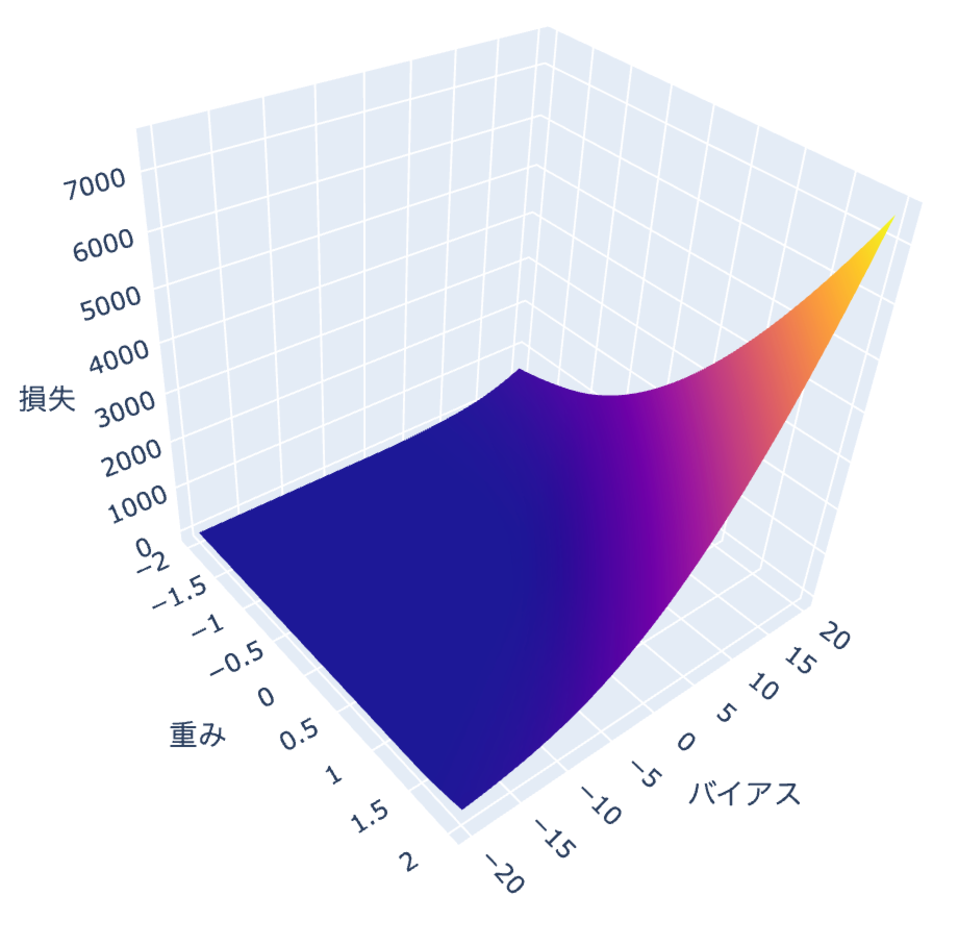
\includegraphics[width=0.7\linewidth]{fig/1-dim-relu-3d.pdf}

    (a) self attention
    \vspace{5mm}

    % 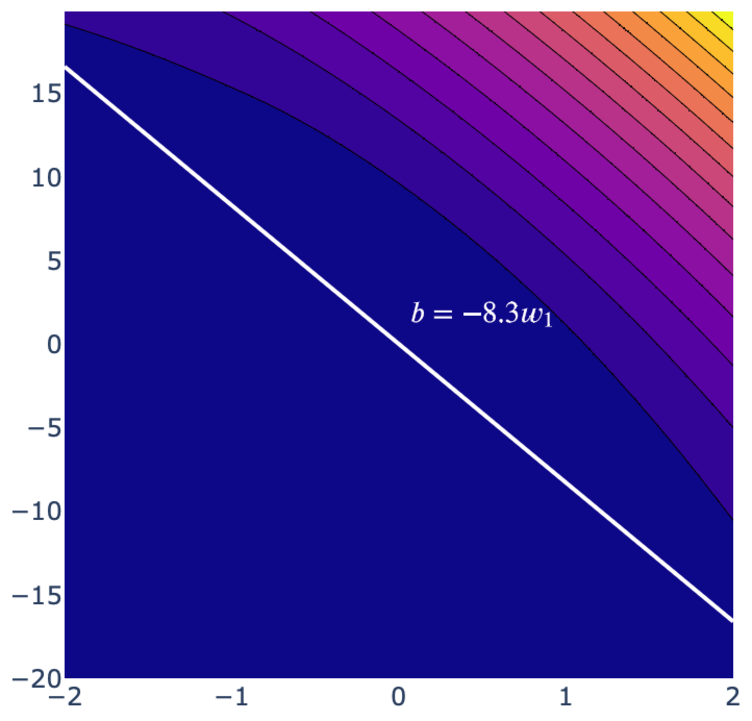
\includegraphics[width=0.7\linewidth]{fig/1-dim-relu-contour.pdf}
    (b) 通常のattention

  \caption{attentionの直観的な概念図}
\label{fig:att-abs}
\end{figure}



\subsubsection{Mask}

\begin{figure}
  \centering
  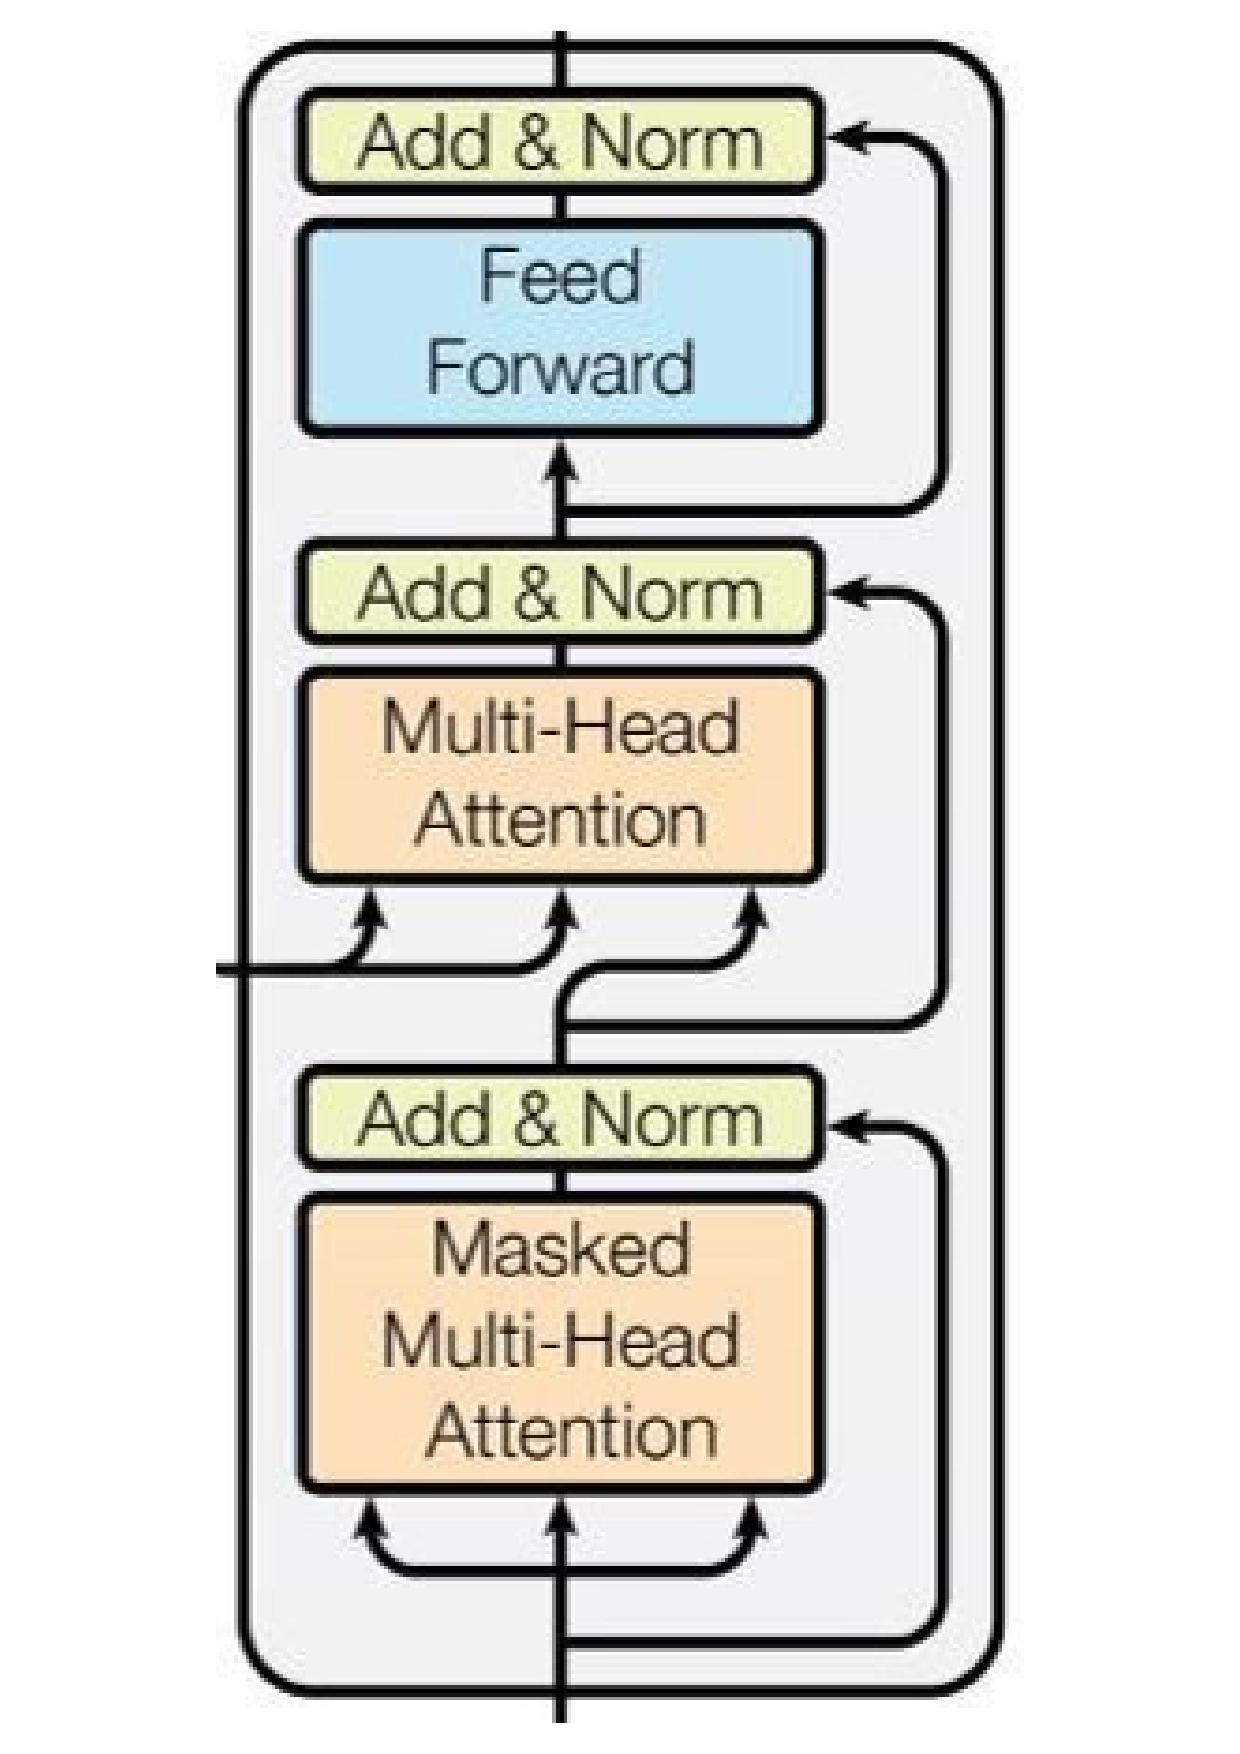
\includegraphics[width=0.5\linewidth]{fig/decoder.pdf}
  \caption{mask}
\label{fig:mask}
\end{figure}

Decoderにおけるself attentionには"Masked Attention"という特殊な名前が付いている。maskとは本来何かを覆い隠したりする意味である。transformerの場合は学習段階において$l$番目のトークン$x_{l+1}$を予測する際に、それ以前のトークン情報のみを予測に使用するように、$l+1$以降のトークンを覆い隠す。言い換えると、mask機能を追加することでtransformerからの出力が式~(\ref{eq:trans})となることを保証している。

\subsubsection{学習}

まずは損失関数を定義する。文章対$(X, Z)$に対してtransformerからの出力$f_\theta(X_i, Z_i)$は
~(\ref{eq:trans})で表されるので、一つのデータ(文章対)に対する損失関数は交差エントロピーを用いて
\begin{equation}
  \label{eq:cross_trans}
  - \sum_{l=0}^{L-1} \log P_\theta(x_{l+1} | Z, x_0, \cdots, x_{l-1} )
\end{equation}
として定義される。
  \label{eq:cross_trans}
訓練データセットに$n$個の文章対$(X_1, Z_1),\ldots, (X_n, Z_n)$が含まれている場合は、損失関数は~(\ref{eq:cross_trans})の単純な足し合わせとして計算すればよい。この損失関数に対して勾配降下法などを用いて最適化をすることで、確率分布$P_\theta(x_{l+1} | Z, x_0, \cdots, x_{l-1} )$を理想の確率分布$P(x_{l+1} | Z, x_0, \cdots, x_{l-1} )$へと近づけていく。 

\subsubsection{推論}
実際に翻訳元の文章$Z = [z_0, z_1, .., z_{L^\prime}]$から翻訳先の文章$X = [x_0, x_1, .., x_{L}]$を生成する場合は、いわゆる\text{\bf{オンライン推論}}が用いられる。オンライン推論では$Z$から一度で翻訳先の文章$X$を生成するのではなく、左から順に一つづつ単語を生成していく。


\begin{equation*}
  \text{具体例}
\end{equation*}


\subsubsection{transformerを用いたモデル}